\documentclass{stdlocal}
\begin{document}
\section{Evaluation and Results} % (fold)
\label{sec:evaluation}
  In section \ref{sec:implementation}, we have implemented scalar and vectorized versions of known PRNGs, namely the MT19937, the Xoroshiro128+, and the MSWS.
  Additionally, unbiased uniform distribution functions for floating-point numbers based on \textcite[\ppno~55-56]{kneusel2018} and \textcite{vigna-xoroshiro} were introduced to completely exploit the vector registers as long as possible.
  The last section \ref{sec:testing_framework} described the implementation of tests and benchmarks to measure the performance of PRNGs concerning statistics and execution time.
  So to prove that the vectorization of PRNGs is indeed improving the performance without reducing statistical quality, we have to apply those benchmarks and analyze their output.

  We have run the benchmarks on two different machines with similar architectures with varying raw computing powers.
  The machines are modern Linux-based $64\appendUnit{bit}$ platforms providing the GCC C++ compiler version 9.2.0 \autocite{gcc}.
  The given C++ code used for including the library and running the tests and benchmarks was compiled with the optimization flags \code{-O3} and \code{-march=native} to guarantee the strongest optimization level.
  Because the generation of random numbers through PRNGs typically does not have to access main memory and can instead completely be run inside the caches of the CPU, specifying the CPU parameters of a target machine will be sufficient to draw conclusions.
  The first machine is a laptop and consists of the \citetitle{intel-kaby-lake-i5} \autocite{intel-kaby-lake-i5} whereas the second machine is a custom desktop computer with an installed \citetitle{intel-kaby-lake-i7} \autocite{intel-kaby-lake-i7}.
  Both systems consist of four cores featuring Hyper-Threading and the SSE/AVX instruction set extensions up to SSE4.2 and AVX2.
  The desktop processor is an high-end performance microprocessor based on the Kaby Lake microarchitecture.
  It operates at a base frequency of $4.2\appendUnit{GHz}$ and a Turbo Boost frequency of up to $4.5\appendUnit{GHz}$ when used in single-core mode.
  The laptop processor is a mobile microprocessor and is also based on an enhanced version of the Kaby Lake microarchitecture.
  It operates at a base frequency of $1.6\appendUnit{GHz}$ and a Turbo Boost frequency of up to $3.4\appendUnit{GHz}$.
  We refer to \textcite{intel-kaby-lake-i5} and \textcite{intel-kaby-lake-i7} for more information.

  \subsection{Statistical Quality} % (fold)
  \label{sub:statistical_quality}
    From a theoretical point of view, interleaving multiple streams of random numbers based on multiple instances of the same generator should not reduce the randomness of the output, such that test suites will be able to measure it.
    Using multiple instances through SSE/AVX vector registers, the state of the vectorized PRNG becomes at least two times as big as the scalar variant.
    According to \textcite{oneill-blog-toobig}, creating a larger state will even make a weak generator stronger concerning its statistical performance.
    On the other hand, \textcite{fog2015} states that the use of multiple instances of the same generator with different seeds can lead to overlapping subsequences.

    For testing the statistical performance, we have used \citetitle{testu01-lib} version 1.2.3 and version 3.31.1 of \citetitle{dieharder}.
    The computation time to run all the tests in the test batteries of TestU01 approximately ranged from $5\appendUnit{s}$ for SmallCrush over $20\appendUnit{min}$ for Crush to $150\appendUnit{min}$ for BigCrush.
    While executing the BigCrush battery, 160 statistics were used to estimate the statistical performance of the generators.
    The execution of all 30 \citetitle{dieharder} tests with different parameters always took several minutes.

    Running the statistical test suites, we could not find any vulnerabilities.
    Neither the scalar nor the vectorized versions of the Xoroshiro128+ and the MSWS systematically failed an empirical test.
    Even a truly random sequence will fail tests from time to time \autocite[\pno~142]{kneusel2018} and so after running the test suites multiple times, we were able to confirm this for our implementations, too.
    Every generator rarely produced test failures that did not follow any pattern.
    We conclude that the usage of multiple instances to vectorize the generators did not reduce their statistical quality.
  % subsection statistical_quality (end)

  \subsection{Performance Improvement} % (fold)
  \label{sub:performance_improvement}
    Applying the designed benchmarks to the implementations of scalar and vectorized PRNGs enables us to evaluate the performance improvement introduced by using vectorization techniques.
    In tables \ref{tab:generation-data-i7} and \ref{tab:monte-carlo-pi-data-i7}, the results for running the generation benchmark and the Monte Carlo π benchmark respectively on the \citetitle{intel-kaby-lake-i7} are given for all the implemented PRNG versions and benchmark scenarios.
    For the MT19937, we have even inserted the data for the STL and Boost implementations to see if the code is indeed outperforming its state-of-art scalar counterparts \autocite{boost,gcc-libstdcpp}.
    All measurements and plots for the \citetitle{intel-kaby-lake-i5} will not be shown in this section to not distract and can be found in the appendix \ref{sec:further_results}.
    Figures \ref{fig:generation-performance-i7} and \ref{fig:generation-speedup-i7} show the respective performance and speedup resulted from running the generation benchmark on the \citetitle{intel-kaby-lake-i7}.
    For the many variants of the Monte Carlo π benchmark, we only show the speed-up in figure \ref{fig:monte-carlo-pi-speedup-i7}.
    The prefix \enquote{2 x} appearing in all figures states that two independent instances of the given generator were used.

    \begin{table}[H]
      \center
      \caption[Generation Benchmark Data for \citetitle{intel-kaby-lake-i7}]{%
        Results achieved by running the generation benchmark on the \citetitle{intel-kaby-lake-i7} at a frequency of $4.51\appendUnit{GHz}$ with all implemented variants of given PRNGs.
        While running the benchmark, $16\appendUnit{GiB}$ of random numbers were generated and temporarily stored in a cache of size $16384\appendUnit{B}$ by iterating $2^{20}$ times over its content.
        During the execution, there were no cache or branch misses.
        The values for cycles, instructions, and IPCs were averaged over the calls to the advancing routine of the respective generator.
      }
      \label{tab:generation-data-i7}
      \footnotesize
      \renewcommand{\arraystretch}{1.2}
      \subimport{tables/}{generation_desktop}
    \end{table}

    \begin{figure}
      \center
      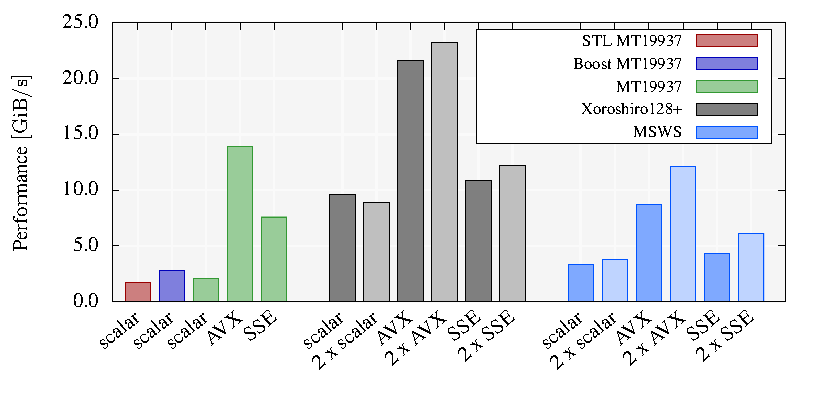
\includegraphics[width=0.95\textwidth]{plots/generation_desktop.pdf}
      \caption[Generation Benchmark Performance for \citetitle{intel-kaby-lake-i7}]{%
        Performance resulting from the generation benchmark running on the \citetitle{intel-kaby-lake-i7} measured in $\mathrm{GiB}$ of random numbers per second for the different variants of the implemented PRNGs.
        For convenience, the performances of the STL and Boost implementation of the MT19937 are shown as well.
        The data can be found in table \ref{tab:generation-data-i7}.
      }
      \label{fig:generation-performance-i7}
    \end{figure}

    \begin{figure}
      \center
      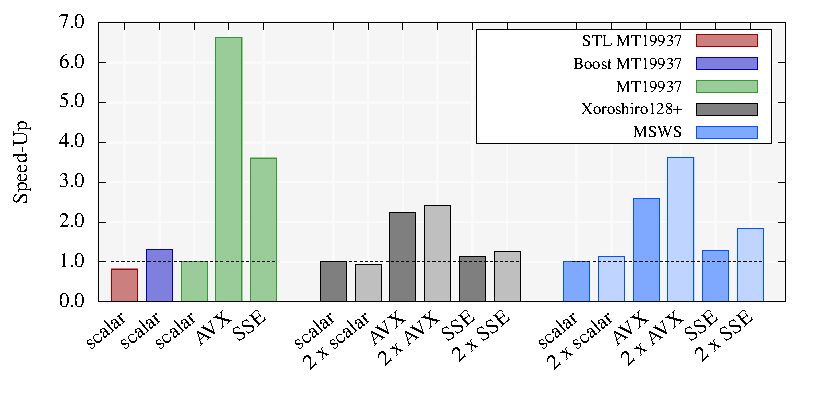
\includegraphics[width=0.95\textwidth]{plots/generation_desktop_speedup.pdf}
      \caption[Generation Benchmark Speed-Up for \citetitle{intel-kaby-lake-i7}]{%
        Speed-up in execution time with respect to the single-instance scalar version resulting from the generation benchmark running on the \citetitle{intel-kaby-lake-i7} for the different variants of the implemented PRNGs.
        For convenience, the speed-ups of the STL and Boost implementation of the MT19937 are shown with respect to our implementation.
        The data can be found in table \ref{tab:generation-data-i7}.
      }
      \label{fig:generation-speedup-i7}
    \end{figure}

    Both target machines consist of similar architectures.
    Comparing the tables \ref{tab:generation-data-i7} and \ref{tab:monte-carlo-pi-data-i7} and the figures \ref{fig:generation-performance-i7}, \ref{fig:generation-speedup-i7}, and \ref{fig:monte-carlo-pi-speedup-i7} to the tables \ref{tab:generation-data-i5} and \ref{tab:monte-carlo-pi-data-i5} and the figures \ref{fig:generation-performance-i5}, \ref{fig:generation-speedup-i5}, and \ref{fig:monte-carlo-pi-speedup-i5} in appendix \ref{sec:further_results} respectively, we see that both architectures exhibit nearly the same speed-up, averaged cycles and averaged instructions.
    Due to differing raw computing power, the execution time and the averaged IPC deviate from each other.
    Therefore we recommend that quantizing the efficiency of a PRNG implementation should use the averaged cycles and instructions to draw conclusions for a given microarchitecture.

    We are mostly interested in the speed-up concerning the execution time of a given benchmark to have a direct comparison between scalar and vectorized generators.
    According to figure \ref{fig:generation-speedup-i7}, in the generation benchmark we were able to achieve a speed-up greater than one for all vectorized versions of PRNGs.

    Our scalar implementation of the MT19937 has already beaten the standard version of the STL but was not able to surpass the Boost implementation.
    However, looking at the speed-up introduced by the usage of SSE and AVX intrinsics, vectorized versions of the MT19937 are more than three times faster by using SSE and more than six times faster by using AVX than their scalar counterparts.
    Vectorizing the MT19937, the best possible theoretical speed-up should be four when used with SSE registers and eight when used with AVX registers.
    The compiler already tries to vectorize the scalar versions so that it is not possible to reach this theoretical bound.
    But this also means that for this scenario the compiler is not able to fully vectorize the scalar implementations automatically, such that manually vectorizing the code is necessary for speeding up the execution.
    In general, the MT19937 speed-ups introduced by SSE and AVX are close to the theoretical maximum.
    Thus, taking the extra effort of vectorizing this generator paid off.
    Additionally, comparing the overall performance of the MT19937 to the other generators by looking at figure \ref{fig:generation-performance-i7} and table \ref{tab:generation-data-i7}, we see that it is competitive.
    For the vectorized versions, the MT19937 is even faster than the MSWS which has a much smaller state size.
    The caching mechanisms of modern computer architecture make it possible to completely keep the state of the MT19937 in the cache while generating new random numbers.
    Furthermore, the transition function is linear and does not exhibit difficult flow or data dependencies as can be seen in figure \ref{fig:mersenne-twister-transition-generation}.
    The advancing routine can therefore exploit modern processor features much better than the implementations of the MSWS or the Xoroshiro128+.
    Due to its non-linearity, the MSWS uses complex functions when advancing its state.
    Looking at figures \ref{fig:xoroshiro-transition-generation} and \ref{fig:msws-transition-generation}, both generators show a higher data dependency which reduces the efficiency of the processor pipeline.
    Hence, the modern design of processors makes it difficult to theoretically analyze the implementations of PRNGs.
    It can even support generators that seem to be slow such that they show a much higher performance than their counterparts.


    The Xoroshiro128+ indeed executes faster by using SSE/AVX intrinsics.
    The SSE variant realizes a speed-up of approximately $1.1$ and the AVX variant a speed-up of $2.2$.
    However, we are much further away from the theoretical bounds than in the case of the MT19937.
    Using SSE, we should reach a speed-up of two, whereas a speed-up of four would be the bound for the AVX version.
    We expect that this time the compiler was much more capable of automatically vectorizing large parts of the code in the generation benchmark.
    If the automatically vectorized code is already exploiting vector intrinsics we cannot hope to reach the theoretical speed-up.
    But instead the manual vectorization was able to further reduce code and data dependencies in the generation benchmark.
    Furthermore, by analyzing latency issues through the use of two independent instances of the generator, we see that in some cases SSE/AVX versions can be further optimized by using the doubled state size to keep the CPU pipeline filled.
    This seems not to be true for the scalar version.
    The implementation of a vectorized Xoroshiro128+ is not a complex procedure.
    As a consequence, even for these smaller speed-ups using vectorization techniques turns out to be profitable.

    The results for the MSWS in the generation benchmark are similar to the results of the Xoroshiro128+.
    The compiler is capable of automatically vectorizing large parts of the code.
    This reduces the possible speed-up reachable by SSE/AVX implementations.
    But this time, we see a strong improvement in performance when using two instances of the MSWS versions.
    In the implementation of the MSWS, we have to carry out a $64\appendUnit{bit}$ multiplication by squaring a number.
    Especially for vector registers, operations needed to compute this result typically feature an acceptable throughput but also a high latency.
    Hence, using the doubled amount of independent states would take advantage of these parameters by keeping the multiplication pipeline filled.
    This also would explain the results.
    Vectorizing the MSWS has been a little bit more complicated than the procedure for the Xoroshiro128+.
    On the other hand, we are getting a slightly better speed-up with the potential for further improvements.
    Figure \ref{fig:generation-performance-i7} shows that the performance of the vectorized MSWS versions is smaller in comparison to the other generators.
    The MSWS seems not to be competitive concerning its execution time, yet.
    Nevertheless, its non-linearity makes it a perfect candidate for more advanced applications with special statistical requirements on used random numbers.

    \begin{table}
      \center
      \caption[Monte Carlo π Benchmark Data for \citetitle{intel-kaby-lake-i7}]{%
        Results achieved by running the Monte Carlo π Benchmark on the \citetitle{intel-kaby-lake-i7} with all implemented variants of given PRNGs and benchmark scenarios.
        While running the benchmark, $10^{8}$ samples in the unit square were used to estimate the value of π.
        It was ensured that the estimation error was small enough according to the calculation at the end of section \ref{sub:monte_carlo_integration}.
        During the execution, there were no cache or branch misses.
        The values for cycles, instructions, and IPCs were averaged over the number of samples in the unit square.
      }
      \label{tab:monte-carlo-pi-data-i7}
      \footnotesize
      \renewcommand{\arraystretch}{1.2}
      \subimport{tables/}{monte_carlo_pi_desktop.tex}
    \end{table}

    \begin{figure}
      \center
      \begin{subfigure}[b]{\textwidth}
        \center
        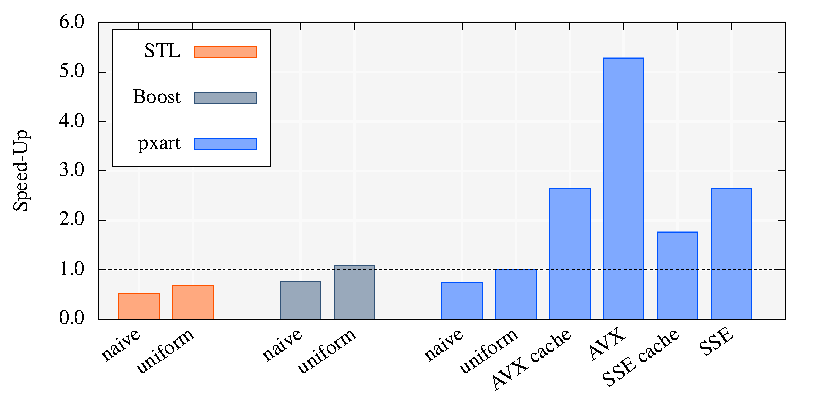
\includegraphics[width=0.95\textwidth]{plots/monte_carlo_pi_desktop_mt19937.pdf}
        \caption{MT19937}
      \end{subfigure}

      \begin{subfigure}[b]{\textwidth}
        \center
        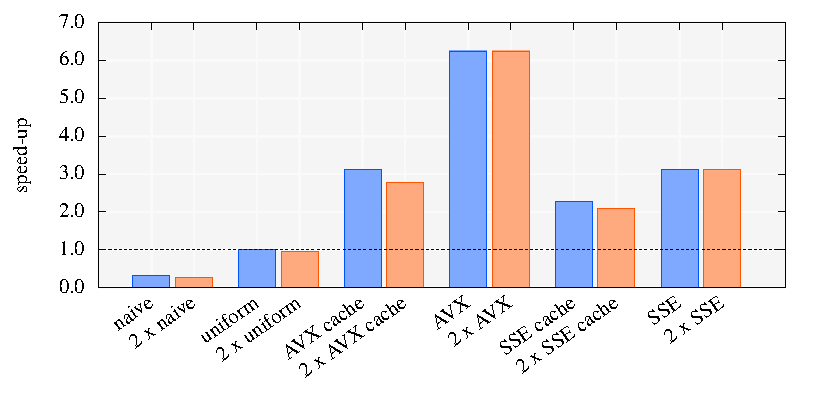
\includegraphics[width=0.95\textwidth]{plots/monte_carlo_pi_desktop_xrsr128p.pdf}
        \caption{Xoroshiro128+}
      \end{subfigure}

      \begin{subfigure}[b]{\textwidth}
        \center
        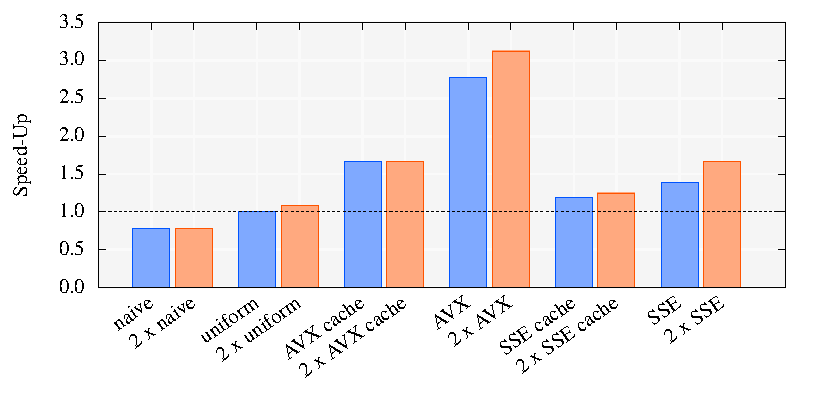
\includegraphics[width=0.95\textwidth]{plots/monte_carlo_pi_desktop_msws.pdf}
        \caption{MSWS}
      \end{subfigure}
      \caption[Monte Carlo π Benchmark Speed-Up for \citetitle{intel-kaby-lake-i7}]{%
        Speed-up in execution time with respect to the single-instance uniform version resulting from the Monte Carlo π benchmark running on the \citetitle{intel-kaby-lake-i7} for the different variants of the implemented PRNGs and benchmark scenarios.
        For convenience, the speed-ups of the STL and Boost implementation of the MT19937 are shown with respect to our implementation.
        The data can be found in table \ref{tab:monte-carlo-pi-data-i7}.
      }
      \label{fig:monte-carlo-pi-speedup-i7}
    \end{figure}

    Looking at the data and plots of the Monte Carlo π benchmark in table \ref{tab:monte-carlo-pi-data-i7} and figure \ref{fig:monte-carlo-pi-speedup-i7}, we first expected to see similar results.
    As before, all the vectorized implementations were able to increase the performance of the program.
    Again, although the MT19937 has a much bigger state, its performance is competitive to the other generators as can be seen in table \ref{tab:monte-carlo-pi-data-i7}.
    Especially the fast uniform distribution function even outperforms the naive scenario for scalar generators in all cases.
    The Monte Carlo π benchmark is a CPU-bound algorithm and therefore we expected such an outcome.
    But this time the compiler was rarely capable of automatically vectorizing the code.
    As a consequence, we could detect much higher speed-ups for the Xoroshiro128+ and MSWS by using vector intrinsics.
    The speed-ups of the MT19937 are reduced.
    Using two instances of independent generators only slightly improves the performance of the MSWS and is not really changing the performance of the Xoroshiro128+.
    We think that this follows from a higher code complexity in the Monte Carlo π benchmark.
    The compiler optimization of the program flow is not as effective as for the generation benchmark.
    However, at the end of each benchmark the estimation of π will printed on the screen which forces the compiler to not remove code that is needed for the computation of π.
    Therefore the Monte Carlo π benchmark did not introduce as much noise to the measurements as the generation benchmark did.
    We conclude that an actual application, like the computation of π, should always be used to measure performance and speed-up of PRNGs.

    Another important point is that we always could reduce the execution time by a factor ranging from $1.2$ to $2.6$ when using a cache without introducing vector intrinsics to the actual benchmark.
    By Amdahl's law, the given speed-ups have to be a lot smaller than the theoretical bounds because a great percentage of the code was not vectorized.
    This means that even in scalar code the usage of vectorized PRNGs improves the overall performance.
    But to completely exploit the speed-up brought by vectorization of PRNGs, developers should consider the usage of SIMD intrinsics in performance-critical parts of their code which are using random numbers.
  % subsection performance_improvement (end)
% section evaluation (end)
\end{document}